\section{Análisis DAFO}  

\begin{figure}[H]
    \centering
    \makebox[\textwidth][c]{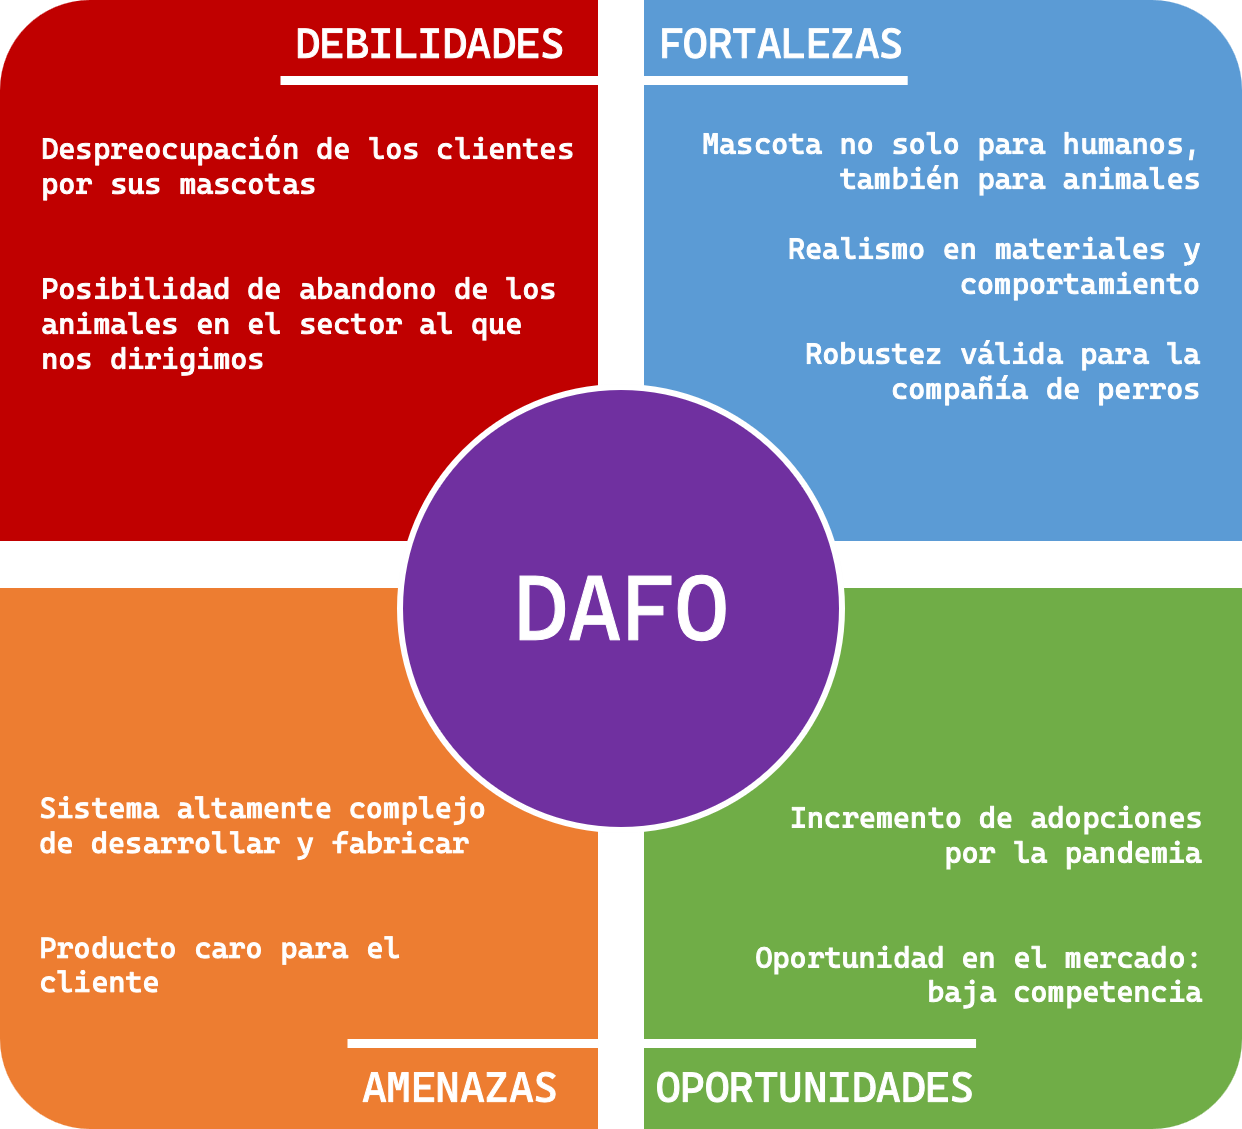
\includegraphics[width=.8\textwidth]{img/dafo.png}}%
\end{figure}

\subsection{Fortalezas}
% • Qué ventajas tiene nuestra empresa (o idea inicial) sobre la competencia (técnicas, de costes, de experiencia, de recursos humanos, .. 
% • Qué elementos perciben nuestros clientes como una fortaleza de empresa 
% • Cual es el know-­‐how de nuestros recursos humanos 
% • Donde está nuestra innovación 

Nosotros proponemos un robot cuadrúpedo que haga que la mascota se encuentra frente ``un igual'', de forma que juegue y se comunique con él al igual que lo haría con otro perro. De esta forma nos diferenciamos de mayoría del mercado, centrado en robots de compañía para humanos y no para mascotas. 

Nuestra investigación de la competencia solo ha encontrado un principal competidor en este segmento. Frente a ellos, su falta de proporciones similares a un perro (el suyo es un robot estilo clásico roomba) y nuestro realismo en olor y textura hará que nuestro modelo alcance más fácilmente el cariño tando de la mascota como del dueño.

\subsection{Debilidades}
% • Qué hace peor nuestra empresa que la competencia 
% • En qué procesos somos más lentos o ineficientes 
% • Qué perciben nuestros clientes como debilidades 
% • Qué aspectos tecnológicos del sector aún no hemos incorporado 
% • Qué nos dificulta adaptarnos a las peFciones de nuestros clientes 

El producto a desarrollar es extremadamente complejo y costoso. Necesitamos proveer de sistemas sensoriales, motores e intelectuales que ``confundan'' a una máquina por un animal (en principio, desde la perspectiva de la mascota). El sistema debe ser robusto y seguro, lo que conlleva mucho tiempo de investigación y testeo.
Todo esto se resume en que contaríamos con un proceso pre-producción largo y caro.

\vspace{\baselineskip}

Esto nos obligará a demostrar con mayor énfasis nuestra propuesta de valor frente a la competencia y las ventajas de la inversión.

\subsection{Oportunidades}
% • Qué tendencias favorables presenta el mercado 
% • Qué necesidades de los clientes no están cubiertas por la competencia 
% • Qué cambios legislaFvos posiFvos se han producido o se prevén 
% • Qué hábitos de vida o de infraestructuras han cambiado y pueden favorecer al sector 

Los robots enfocados a perros en la actualidad carecen de facultades realistas que permitan que el animal empatice de forma más profunda. La mayoría vagamente pasan del umbral de ``juguetes con ruedas'' y buscan más paliar el servicio de proporcionar comida que de acompañar. Además sabemos que una gran parte de los dueños de mascotas están dispuestos a gastar grandes cantidades de dinero por el bienestar tanto físico como emocional del animal.

\vspace{\baselineskip}

Por otro lado, la masiva adopción de perros por la pandemia en hogares/familias que no estaban preparados para ellos a largo plazo acaba con los animales gran parte del día solos en casa o abandonados. Ya que tras el levantamiento de los confinamientos los dueños vuelven a la rutina y están poco tiempo presentes en la casa. Nuestro robot mascota aporta entretenimiento y compañía para los animales durante estas horas de ausencia.

% https://www.kickstarter.com/projects/51244428/mia-a-friendly-robot-for-cats-and-dogs-by-kolony-r

\subsection{Amenazas}
% • Qué cambios tecnológicos que yo no dispongo están sucediendo en el mercado 
% • Qué hábitos de consumo se prevén que puedan reducir el mercado 
% • Qué tendencias demográficas pueden perjudicar al sector 
% • Cual es la situación del sector financiero 
% • Qué acuerdos internacionales pueden perjudicarnos 

La posibilidad de abandono de las mascotas en los hogares de estos posibles clientes puede reducir significativamente el mercado. Adicionalmente, la gran cantidad de financiación necesaria y lo complejo del desarrollo puede dejarnos sin recursos económicos antes de lanzar el robot en producción.